\chapter{Interactions and color display. }
\minitoc  


\section{Interacting with objects}
One very important aspect of MorphoDig's design is that most interactions or modifications of opened objects can only be done when these objects are \textbf{selected}. 
Selected surfaces (free-form surfaces, landmarks and flags) are always drawn in ``grey". Regarding volumetric objects, selected ones appear with a bounding box, while unselected ones to not exhibit such bounding boxes. See Fig. \ref{selected_unselected} p.\pageref{selected_unselected}.
All currently opened objects can be selected by pressing CTRL+A. All currently opened objects can be unselected by pressing CTRL+D. Objects can also be selected/unselected using the right mouse button, depending on the currently active interaction mode (see below).


\begin{figure}
  \centering
  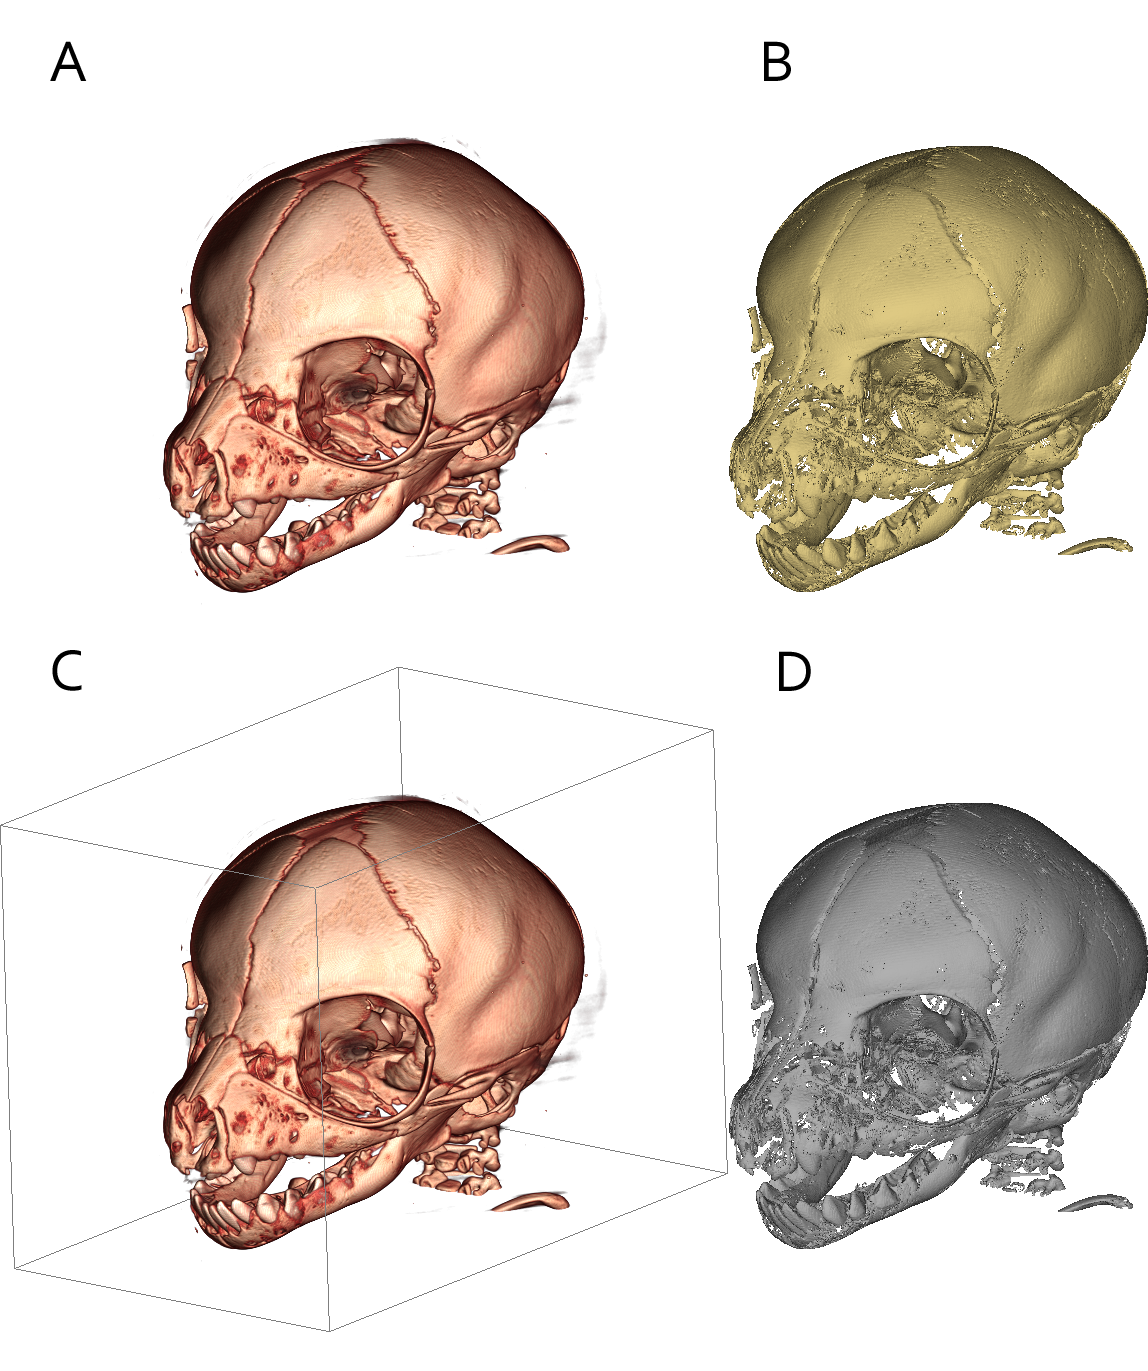
\includegraphics[scale=0.39]{images/04/selected_unselected2.png} 
	\caption{\textbf{A} unselected volumes have no bounding box. \textbf{B} unselected surfaces are usually not drawn grey. \textbf{C} selected volumes exhibit a bounding box. \textbf{D} selected surfaces are drawn grey.}
\label{selected_unselected}
 
\end{figure}

\section{Interactions modes}

See Fig. \ref{gui} p.\pageref{gui} to find the location of the "Interaction modes" controls in the main Window.
\subsection{Camera mode}
  
\includegraphics[scale=0.7]{images/04/camera_mode.png}``Camera mode" is the default interaction mode, and is active on startup. When active, left and middle mouse button drags result in camera rotation/translation, respectively. Right mouse button drag results in object selection/unselection. Pressing "ESC" switches between object mode and camera mode.
\subsection{Object mode}
   
\includegraphics[scale=0.7]{images/04/move_mode.png}When active, left and middle mouse button drags result in object rotation/translation, respectively. Right mouse button drag results in object selection/unselection. Pressing "ESC" switches between object mode and camera mode.
\subsection{Landmark mode}
  
\includegraphics[scale=0.7]{images/04/Landmarks2.png}When active, only landmarks can be selected/unselected via right mouse button drag. This mode is useful when editing/placing landmarks. Left and middle mouse button drags result in camera rotation/translation, respectively.

\section{Landmark setting modes}
Landmarks can be set on surfaces by pressing ``L" + left mouse click. 
Four series of landmarks can be set with MorphoDig: ``normal" landmarks, ``target" landmarks, ``curve node" landmarks and ``curve handle" landmarks. Additionally a fourth special landmark series (``flag" landmarks) can be used to label surface structures. 

\subsection{Normal landmark mode}	
Press ``
\includegraphics[scale=0.7]{images/04/normal_landmarks.png}" to activate this mode (this mode is active by default)

\subsection{Target landmark mode}	
Press ``
\includegraphics[scale=0.7]{images/04/target_landmarks.png}"  to activate this mode

\subsection{Curve node mode}	
Press ``
\includegraphics[scale=0.7]{images/04/curve_nodes.png}" to activate this mode 

\subsection{Curve handle mode}	
Press ``
\includegraphics[scale=0.7]{images/04/curve_handles.png}"  to activate this mode


\subsection{Flag landmark mode}	
Press ``
\includegraphics[scale=0.7]{images/04/flag_landmarks.png}" to activate this mode


 \section{Unselected surfaces color display}
See Fig. \ref{gui} p.\pageref{gui} to find the location of the "Array controls", which impact the color display of the surfaces.
 A given unselected surface can be colored: 
\begin{itemize}
\item using a uniform ``solid" color (Fig. \ref{4color_modes}-A p.\pageref{4color_modes}). Scalar display mode must be deactivated or active array combo box set to ``Solid color" (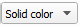
\includegraphics[scale=0.5]{images/04/scalarcombo_solidcolor.png})
\item	according to the scalar values (= numbers) associated at the vertices (Fig. \ref{4color_modes}-B p.\pageref{4color_modes}). Array display mode button must be pressed (
\includegraphics[scale=0.7]{images/04/show_color_scale.png}), and a Scalar array must be selected (ex:
\includegraphics[scale=0.5]{images/04/scalarcombo_scalar.png}). The way scalar arrays are translated into colors can be set up using color "Lookup tables" (LUT), also referred to as color transfer functions. The "Scalar rendering options" window can be opened by clicking on "
\includegraphics[scale=0.7]{images/04/color_scale_edit.png}". 
\item according to the tag values (= integers) associated to the vertices (Fig. \ref{4color_modes}-C p.\pageref{4color_modes}). Array display mode button must be pressed (
\includegraphics[scale=0.7]{images/04/show_color_scale.png}), and a Tag array must be selected (ex:
\includegraphics[scale=0.5]{images/04/scalarcombo_tag.png}). The way Tag arrays are translated into colors can be set up using color "Lookup tables" (LUT), also referred to as color transfer functions. The "Tag options" window, in which lookup tables associated to tag arrays can be edited, can be opened by clicking on "
\includegraphics[scale=0.7]{images/04/tag_edit.png}"
\item	according to RGB values directly associated to the vertices (Fig. \ref{4color_modes}-D p.\pageref{4color_modes}). Array display mode button must be pressed (
\includegraphics[scale=0.7]{images/04/show_color_scale.png}), and a RGB array must be selected (ex:
\includegraphics[scale=0.5]{images/04/scalarcombo_rgb.png}) 
\end{itemize}

\begin{figure}
  \centering
  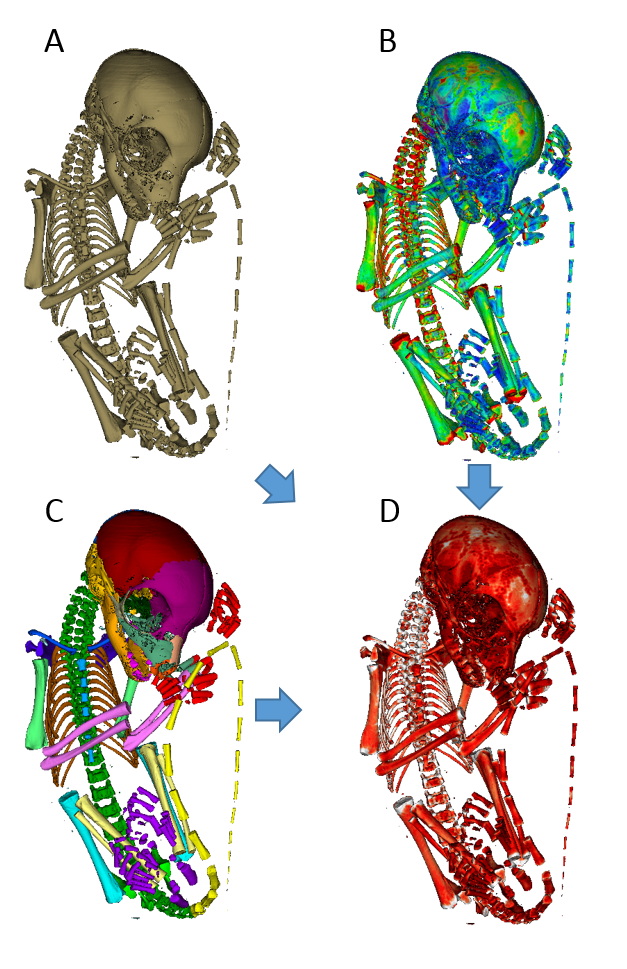
\includegraphics[scale=0.39]{images/04/4color_modes.png} 
	\caption{Color modes for a given surface. Single surface representation of the skeleton of a newborn \textit{Lemur catta}. A: "Solid color mode" mode : a uniform color is used to represent the whole surface. B: "Scalar array" representation mode. Numbers (here bone thickness) are associated to each vertex of the surface, and are rendered using a color map. C: "Tag array". Integers are associated to each vertex  (here different integer values are associated to different groups of bones), and a color map is used  to colorize the specimen. D : "RGB array" : red, green, blue and transparency information is directly associated to each vertex: no color map is used in that case. In MorphoDig, RGB arrays can be produced out of solid color information, scalar arrays and tag arrays. PLY file produced via surface scans often contain surch RGB information.}
\label{4color_modes}
 
\end{figure}